\section{State-of-the-art Architecture}
The custom version of VGG network depicted in Figure~\ref{fig:state_of_the_art} achieves the state-of-the-art accuracy of 84.9\% on the FER+ dataset. This network has 10 convolutional layers, interleaved with max pooling and dropout layers. More concretely, there are 2 convolutional layers after the input with 64 filters of size $3\times 3$. After those 2 layers, max pooling and dropout layers with dropout rate of 25\% follow. The structure repeats but changes in the number of feature maps per convolutional layer and the number of convolutional layers. After the 10 convolutional layers 2 dense layers are added each with 1024 nodes and each followed by a dropout rate of 50\%. The final dense layer has 8 nodes equal to the number of classes and is followed by a softmax layer that gives the probability for every emotion category. This architecture is trained from scratch, and during training they augment the data on the fly by applying simple affine transformations. Since the dataset is annotated by 10 taggers, they could generate a probability distribution for every image where the probability for a specific emotion is equal to the number of annotators that voted for this emotion divided by the total number of annotators which is 10. So for the $n^{th}$ image in the dataset the crowdsourced emotion distribution is $p_{k}^{n}$ with $k=1...8$, where:
$$\sum_{k=1}^{8}p_k^{n}=1$$

The loss function used for training this architecture is the categorical cross entropy given by:
\begin{center}
$$L(t) = -\sum_{n=1}^{N}\sum_{k=1}^{8}p_{k}^{n}\log q_{k}^{n}$$\\
\text{where~$p_{k}^{n}$ is the probability given by the annotators for the image $n$ and}
\text{for the emotion $k$ and $q_{k}^{n}$ is the probability given by the softmax layer}
\text{ for the same image and emotion.}
\end{center}

The metric that they used to evaluate their model is the accuracy which is the percentage of correctly classified instances and is given by the following formula:
\begin{center}
$Accuracy = \frac{TP + TN}{N}$\\
\text{where $TP$ is the true positives, $TN$ is the true negatives}
\text{and $N$ the number of images in the dataset}
\end{center}

\begin{figure}[H]
    \begin{center}
    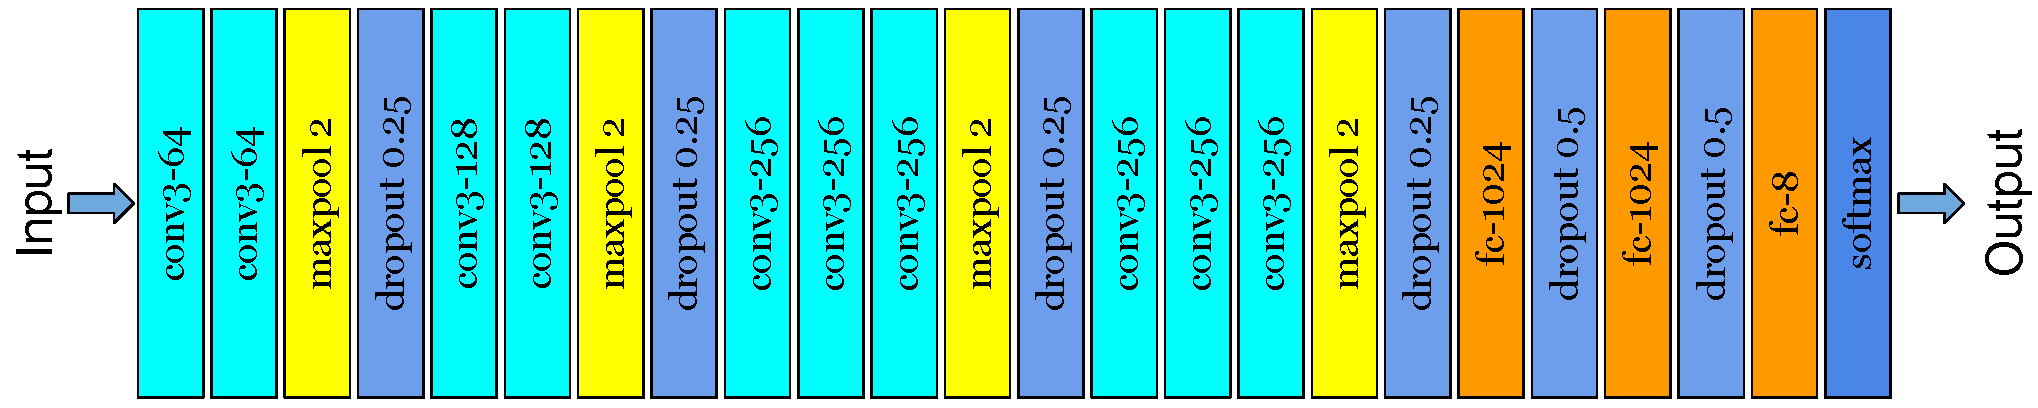
\includegraphics[width=0.8\textwidth]{images/state_of_the_art.pdf}
    \end{center}
    \caption{State of the Art Architecture} \label{fig:state_of_the_art}
\end{figure}

In this project, we experiment with the latest deep convolutional neural networks as discussed in chapter~\ref{ch:architectures} by training them from scratch with the FER+ dataset. Also we experiment with the two most popular techniques in Computer Vision, namely Transfer learning and Multi-task learning that are beneficial in many cases discussed in chapters~\ref{ch:transfer learning} and~\ref{ch:multi-task learning} respectively. Furthermore, we use Action Units discussed in section~\ref{ch:introduction} as additional information which encode facial muscle movement and can help to improve the performance. Also as~\cite{barsoum2016training} did, we apply data augmentation to our dataset by applying geometric transformations to the images. Data augmentation is a methodology that generates new data from our existing dataset. By using this technique the model is able to generalise well during the test phase, and also is very useful to combat imbalanced datasets which is the case for the FER+ dataset. More concretely we use the following transformations for all the experiments:

\begin{itemize}
  \item Scaling
  \item Rotation
  \item Translation
  \item Horizontal flipping
\end{itemize}

Also in every architecture we experiment with different values for the following hyperparameters:

\begin{itemize}
  \item Optimizer (Adam~\cite{kingma2014adam}, Stochastic gradient descent)
  \item Learning rate (0.1, 0.01, 0.001, 0.0001)
  \item Batch size (32, 64, 128)
  \item Dropout rate (0.25, 0.3, 0.5)
  \item Decay (1e-4, 1e-5, 1e-6)
\end{itemize}

Finally during the training phase we use as the loss function the \textit{categorical cross entropy} and the \textit{accuracy} as the metric in order to have a direct comparison with the state of the art accuracy. 

\section{VGG-13}
VGG13 (Figure~\ref{fig:vgg13_16_19}) is the shallowest version of the VGG architecture with 10 convolutional layers. The word \textit{conv3-512} from the figure's box means that the convolutional layer uses 512 filters of size $3\times 3$. The word \textit{maxpool2} means that the size of max pooling layer is of size $2\times 2$, and the word \textit{fc-4096} means that the layer is fully connected with 4096 nodes. The hyperparameters that achieve the best test accuracy are:

\begin{itemize}
  \item Optimizer: Stochastic gradient descent
  \item Learning rate: 0.01
  \item Batch size: 128
  \item Dropout rate: Not available in this architecture
  \item Decay: 1e-6
\end{itemize}

The result can be found in table~\ref{tab:cnn_accuracies}.

\begin{figure}[]
    \begin{center}
    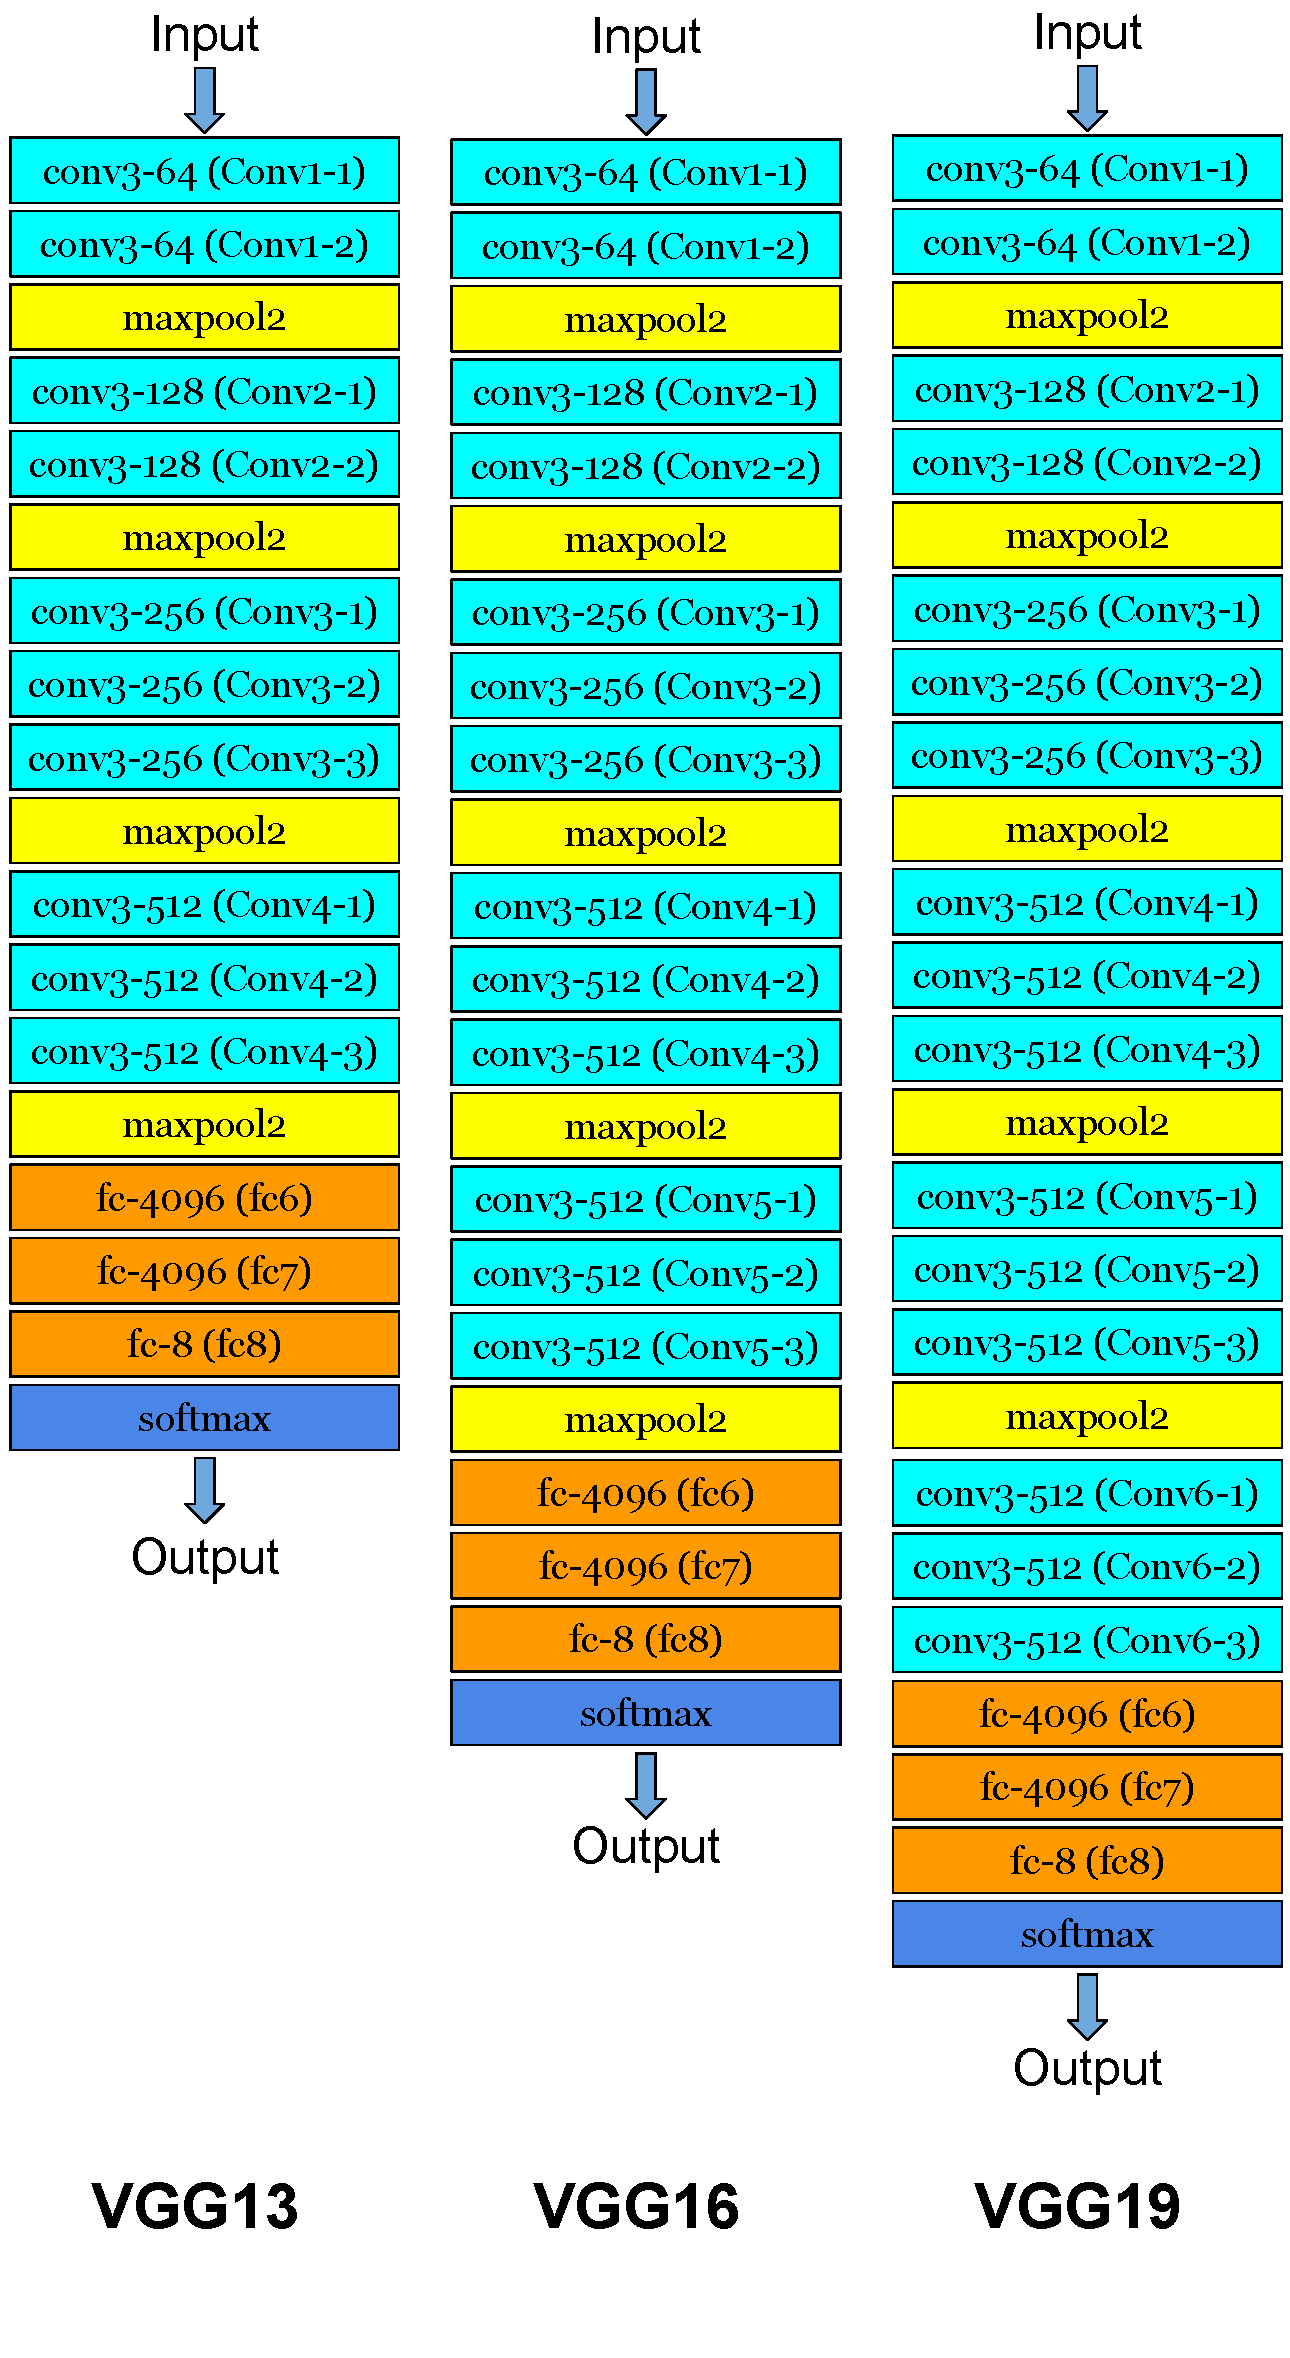
\includegraphics[width=0.8\textwidth]{images/VGG13_16_19.pdf}
    \end{center}
    \caption{VGG Architectures} \label{fig:vgg13_16_19}
\end{figure}

\section{VGG-16}
We try a deeper version of VGG architecture with 3 additional convolutional layers with 512 feature maps each depicted on Figure~\ref{fig:vgg13_16_19}. 

\begin{itemize}
  \item Optimizer: Stochastic gradient descent
  \item Learning rate: 0.01
  \item Batch size: 128
  \item Dropout rate: Not available in this architecture
  \item Decay: 1e-6
\end{itemize}

The result can be found in table~\ref{tab:cnn_accuracies}.

\section{VGG-19}
We try the deepest version of the VGG architecture with 16 convolutional layers and 3 fully connected layers depicted on Figure~\ref{fig:vgg13_16_19}.

\begin{itemize}
  \item Optimizer: Stochastic gradient descent
  \item Learning rate: 0.01
  \item Batch size: 128
  \item Dropout rate: Not available in this architecture
  \item Decay: 1e-6
\end{itemize}

The result can be found in table~\ref{tab:cnn_accuracies}.

\section{ResNet-18}
We evaluate a 18-layer residual network. See Figure~\ref{fig:resnets.png} for details concerning the architecture.

\begin{itemize}
  \item Optimizer: Adam
  \item Learning rate: 0.001
  \item Batch size: 128
  \item Dropout rate: Not available in this architecture
  \item Decay: 0.0
\end{itemize}

The result can be found in table~\ref{tab:cnn_accuracies}.

\section{ResNet-34}
We evaluate a 34-layer residual network. See Figure~\ref{fig:resnets.png} for details concerning the architecture.

\begin{itemize}
  \item Optimizer: Adam
  \item Learning rate: 0.001
  \item Batch size: 128
  \item Dropout rate: Not available in this architecture
  \item Decay: 0.0
\end{itemize}

The result can be found in table~\ref{tab:cnn_accuracies}.

\section{ResNet-50}
We evaluate a 50-layer residual network. See Figure~\ref{fig:resnets.png} for details concerning the architecture.

\begin{itemize}
  \item Optimizer: Stochastic gradient descent
  \item Learning rate: 0.001
  \item Batch size: 128
  \item Dropout rate: Not available in this architecture
  \item Decay: 0.0
\end{itemize}

The result can be found in table~\ref{tab:cnn_accuracies}.

\begin{figure}[]
    \begin{center}
    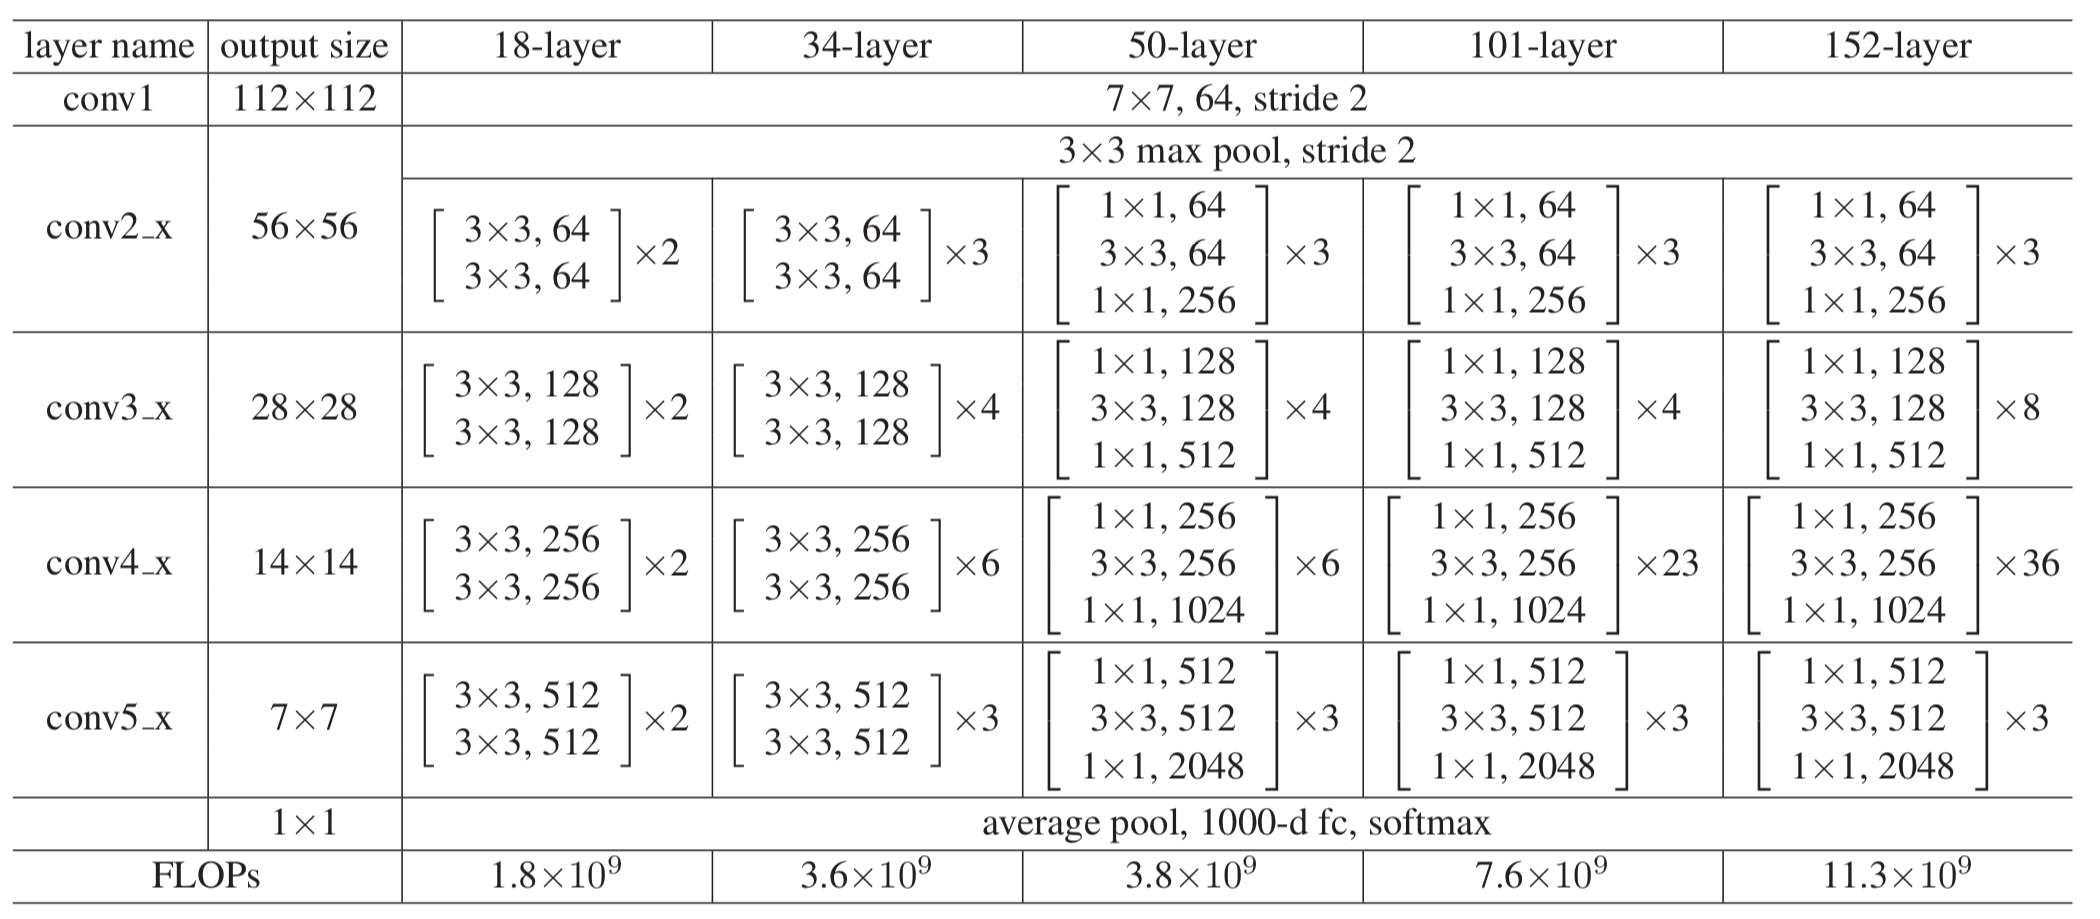
\includegraphics[width=0.8\textwidth]{images/resnets.png}
    \end{center}
    \caption{Examples of conversion from grayscale to RGB images} \label{fig:resnets.png}
\end{figure}


\section{DenseNet}
Unfortunately we couldn't experiment with this architecture, since it is very computationally expensive and as a result we couldn't train with a batch size larger than 8.

\section{Wide ResNet}
As discussed in chapter~\ref{ch:architectures} Wide ResNet is a novel architecture that decreases the depth of the network while increasing the width of the convolutional layers. By doing this, we can achieve superior performance over the commonly used very deep and thin networks. After many experiments, we end up with an architecture that is 28 layers deep and is 4 times wider than the common ResNet network. By using this network with the following hyper-parameters we achieved state-of-the-art accuracy to our main dataset.

\begin{itemize}
  \item Optimizer: Stochastic gradient descent
  \item Learning rate: 0.1
  \item Batch size: 128
  \item Dropout rate: 0.3
  \item Decay: 0.0
\end{itemize}

The result can be found in table~\ref{tab:cnn_accuracies}.

\section{Transfer Learning}
As discussed in chapter~\ref{ch:transfer learning} there are 2 ways to perform transfer learning, either you use a pre-trained network to extract features that you feed to a classifier to do the classification, or you use the entire pre-trained architecture, freeze some layers and train the rest of the layers. In our experiments we use architectures that are trained on ImageNet and for face recognition task namely VGGFace~\cite{Parkhi15}. 

\subsection{Using pre-trained CNN features}
Despite the fact that CNN are complex models and many details on how these models work remain a mystery, we know that the convolutional layers closer to the input represent low-level image features such as edges, while higher level convolutional layers represent more complex features such as faces, emotions, etc. The final fully connected layers are generally assumed to contain information that is relevant to the task. So the idea of this method as discussed in chapter~\ref{ch:transfer learning} is to use the CNN as a feature generator that extracts a set of features for every input. Those features are fed to a Linear SVM classifier that does the classification.

\subsubsection{VGG16 pretrained on ImageNet}
We use the pre-trained on ImageNet VGG16 network depicted on Figure~\ref{fig:vgg13_16_19} as the feature generator. Since the original network was trained with images of dimensions $224\times 224 \times 3$, we have to convert our images from grayscale to rgb and resize them from $48\times 48$ pixels to $224\times 224$ pixels. Examples of this conversion are depicted on Figure~\ref{fig:gray_rgb.pdf}. From the \textit{fc6} layer we extract 4096 features that we use to train an SVM classifier. Furthermore we extract features from the ~\textit{fc7} layer and again we train an SVM classifier. The algorithm is depicted in Figure~\ref{fig:SVM_fc6_fc7.pdf}. The results can be found in Table~\ref{tab:transfer_learning_accuracies}.

\begin{figure}[]
    \begin{center}
    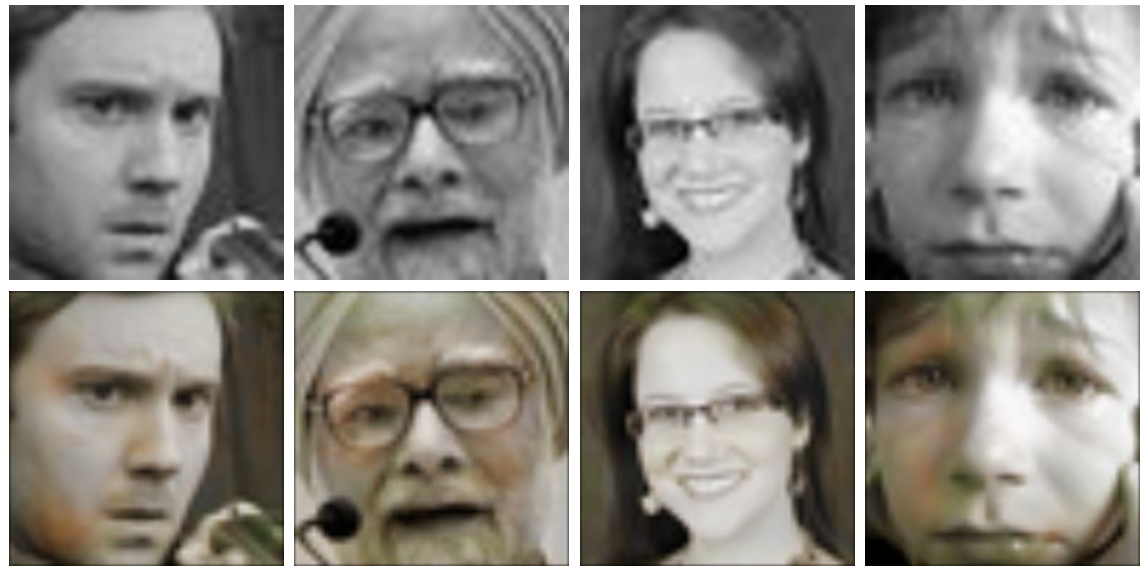
\includegraphics[width=0.8\textwidth]{images/gray_rgb.pdf}
    \end{center}
    \caption{Examples of conversion from grayscale to RGB images} \label{fig:gray_rgb.pdf}
\end{figure}

\begin{figure}[H]
    \begin{center}
    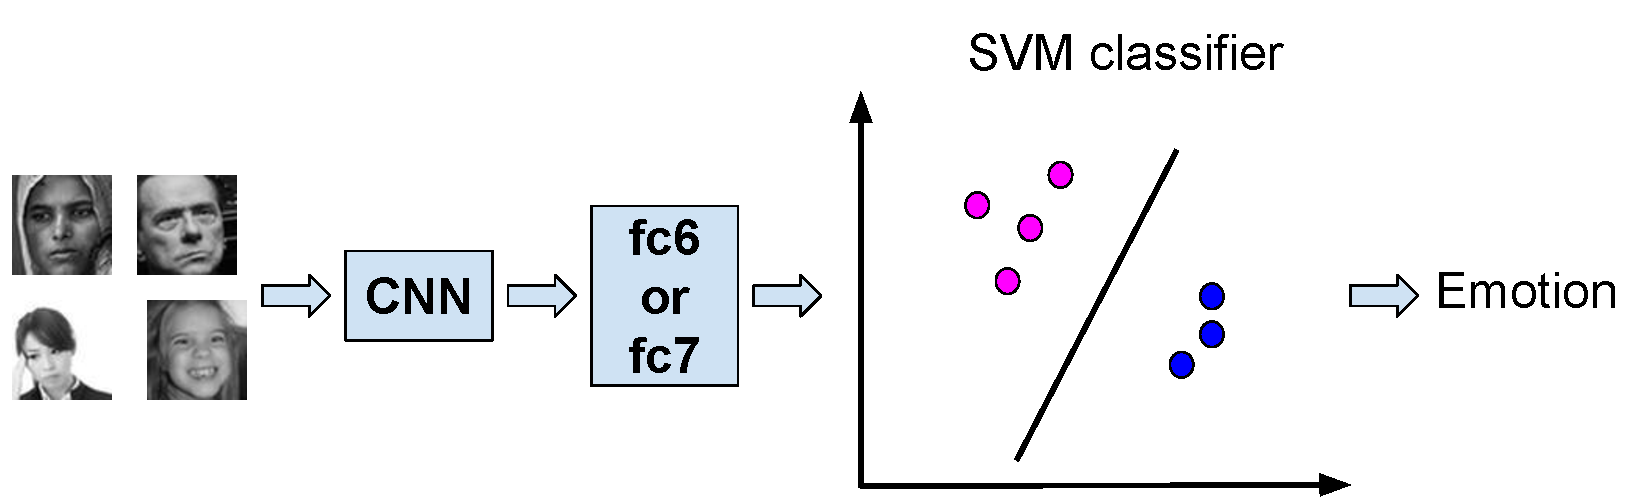
\includegraphics[width=0.8\textwidth]{images/SVM_fc6_fc7.pdf}
    \end{center}
    \caption{Illustration of the proposed method for transfer learning.} \label{fig:SVM_fc6_fc7.pdf}
\end{figure}


\subsubsection{ResNet50 and InceptionV3 pretrained on ImageNet}
As before we use these pre-trained networks to extract features from the last layer and follow the same methodology as before. The results can be found in Table~\ref{tab:transfer_learning_accuracies}.


\subsubsection{VGG16 pretrained for face recognition}
We use the pre-trained for face recognition VGG16 network and follow the same methodology as with the VGG16 model pre-trained on ImageNet. Again we extract features from the \textit{fc6} and \textit{fc7} layers and train an SVM classifier. The results can be found in Table~\ref{tab:transfer_learning_accuracies}.

\subsection{Fine-tuning}

\subsubsection{VGG16 pretrained on ImageNet and for Face Recognition}
In this workflow we use the pre-trained on ImageNet and for Face Recognition VGG16 networks. The idea is to not train from scratch the entire network but to fine-tune some of the higher-level layers during backpropagation, while keeping the rest of the layers intact. As discussed in chapter~\ref{ch:transfer learning} this is motivated by the fact that the earlier layers of a convolutional neural network learn some generic features (edges, blobs, colors, etc.) that are useful to many tasks. So we experiment by freezing two different sets of convolutional layers as depicted in Figure~\ref{VGG16_Finetuning}.

\begin{figure}[]
    \begin{center}
    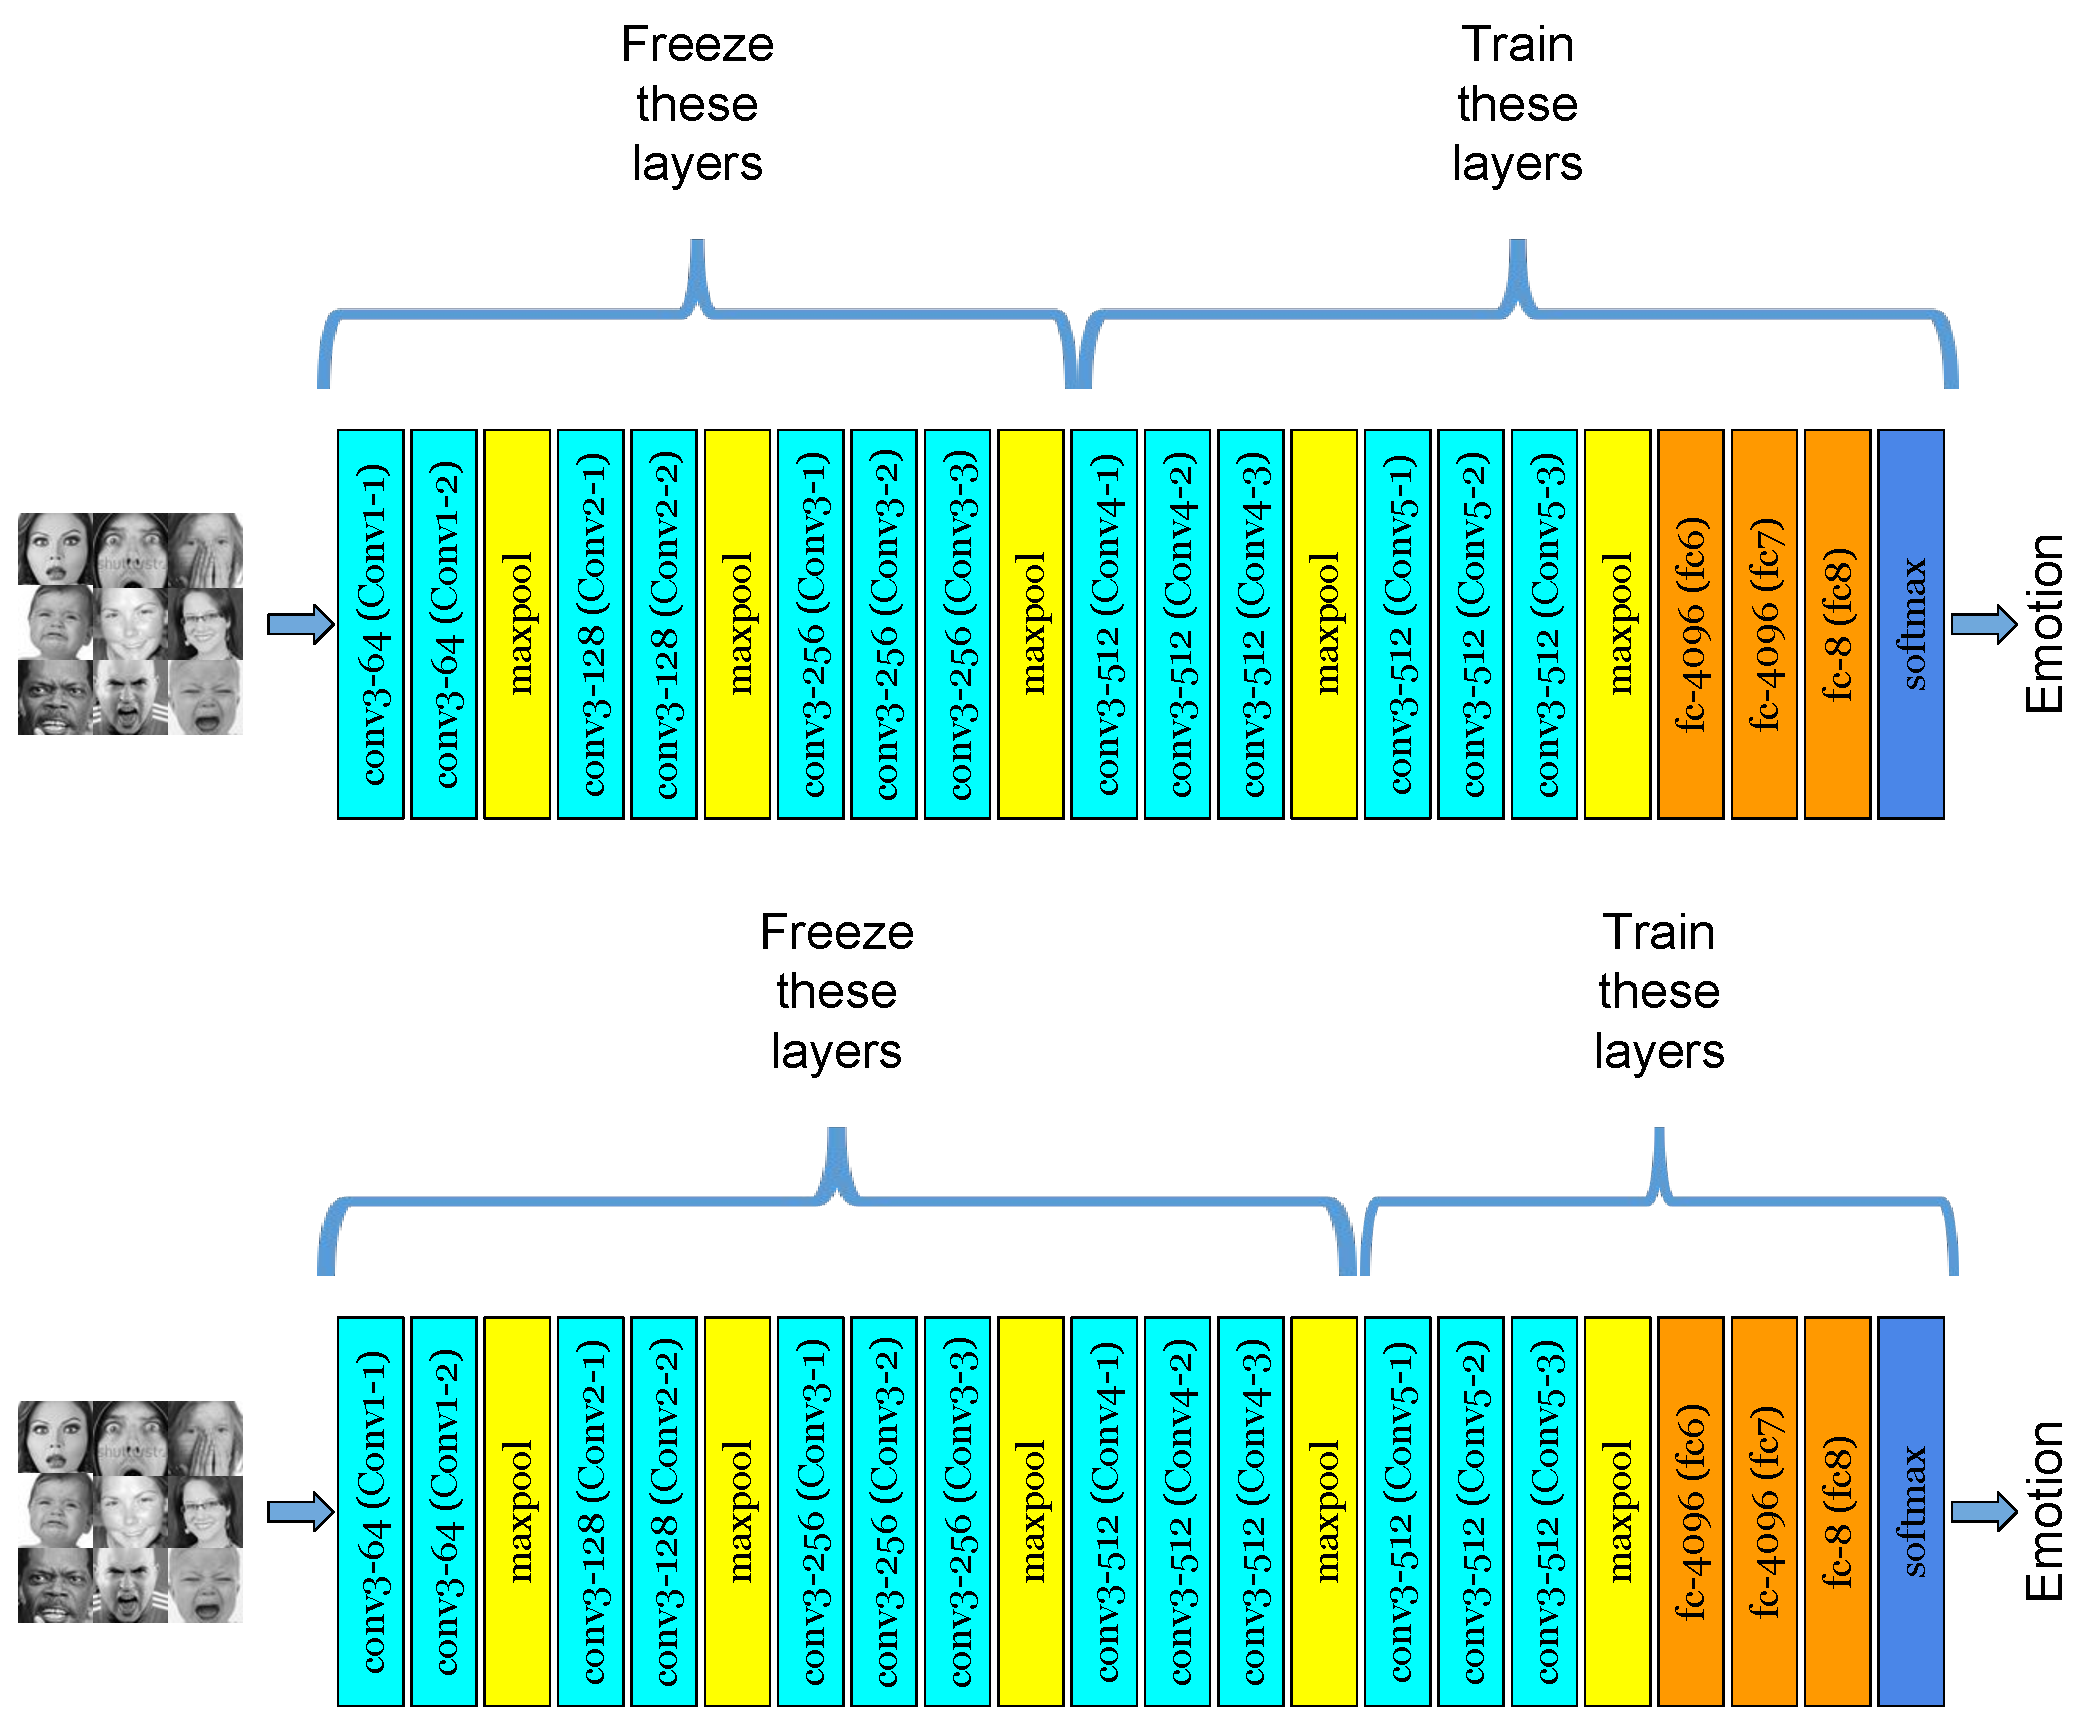
\includegraphics[width=0.8\textwidth]{images/VGG16_Finetuning.pdf}
    \end{center}
    \caption{Fine-tuning VGG16 architecture.} \label{VGG16_Finetuning}
\end{figure}


\section{Multi-task Learning}
In transfer learning we care about getting good results on our target domain. On the contrary in multi-task learning the goal is to exploit the synergy effect between closely related tasks and improve the accuracy on all tasks. The starting point for doing multi-task learning is the architecture that achieved state-of-the-art result on the FER+ dataset depicted on Figure~\ref{fig:state_of_the_art}. After many experiments between we conclude to the architecture depicted on Figure~\ref{fig:multitask_real_1}. The network has 3 branches as the number of tasks. We train this network with 2 different datasets. The branch that does the emotion recognition is trained with the FER+ dataset, and the other 2 branches with the IMDB-WIKI 500+ described on Chapter~\ref{ch:datasets}. The result of this method can be found in Table~\ref{tab:multitask_learning}.

\section{Discussion on the Results}
As we can see from the tables~\ref{tab:cnn_accuracies},~\ref{tab:transfer_learning_accuracies}, and~\ref{tab:multitask_learning}, training deep neural networks from scratch achieves much higher performance than transfer learning and multi-task learning. Also we observe that as we increase the depth of VGG and ResNet architectures the performance degrades. This is also obvious by the performance of GoogLeNet architecture which is a very deep network. Maybe this is caused by the fact that our dataset is small for these deep architectures, and that's why a wider and shallower network like Wide ResNet can achieve such a good performance. Transfer learning doesn't work in our case. Maybe this is caused by the fact that our dataset consists of low resolution $48\times 48$ pixels images that need to be resized to $224\time 224$ pixels and converted to images with 3 channels. As depicted in Figure~\ref{fig:gray_rgb.pdf} the conversion is far from the ground truth.

\begin{figure}[]
    \begin{center}
    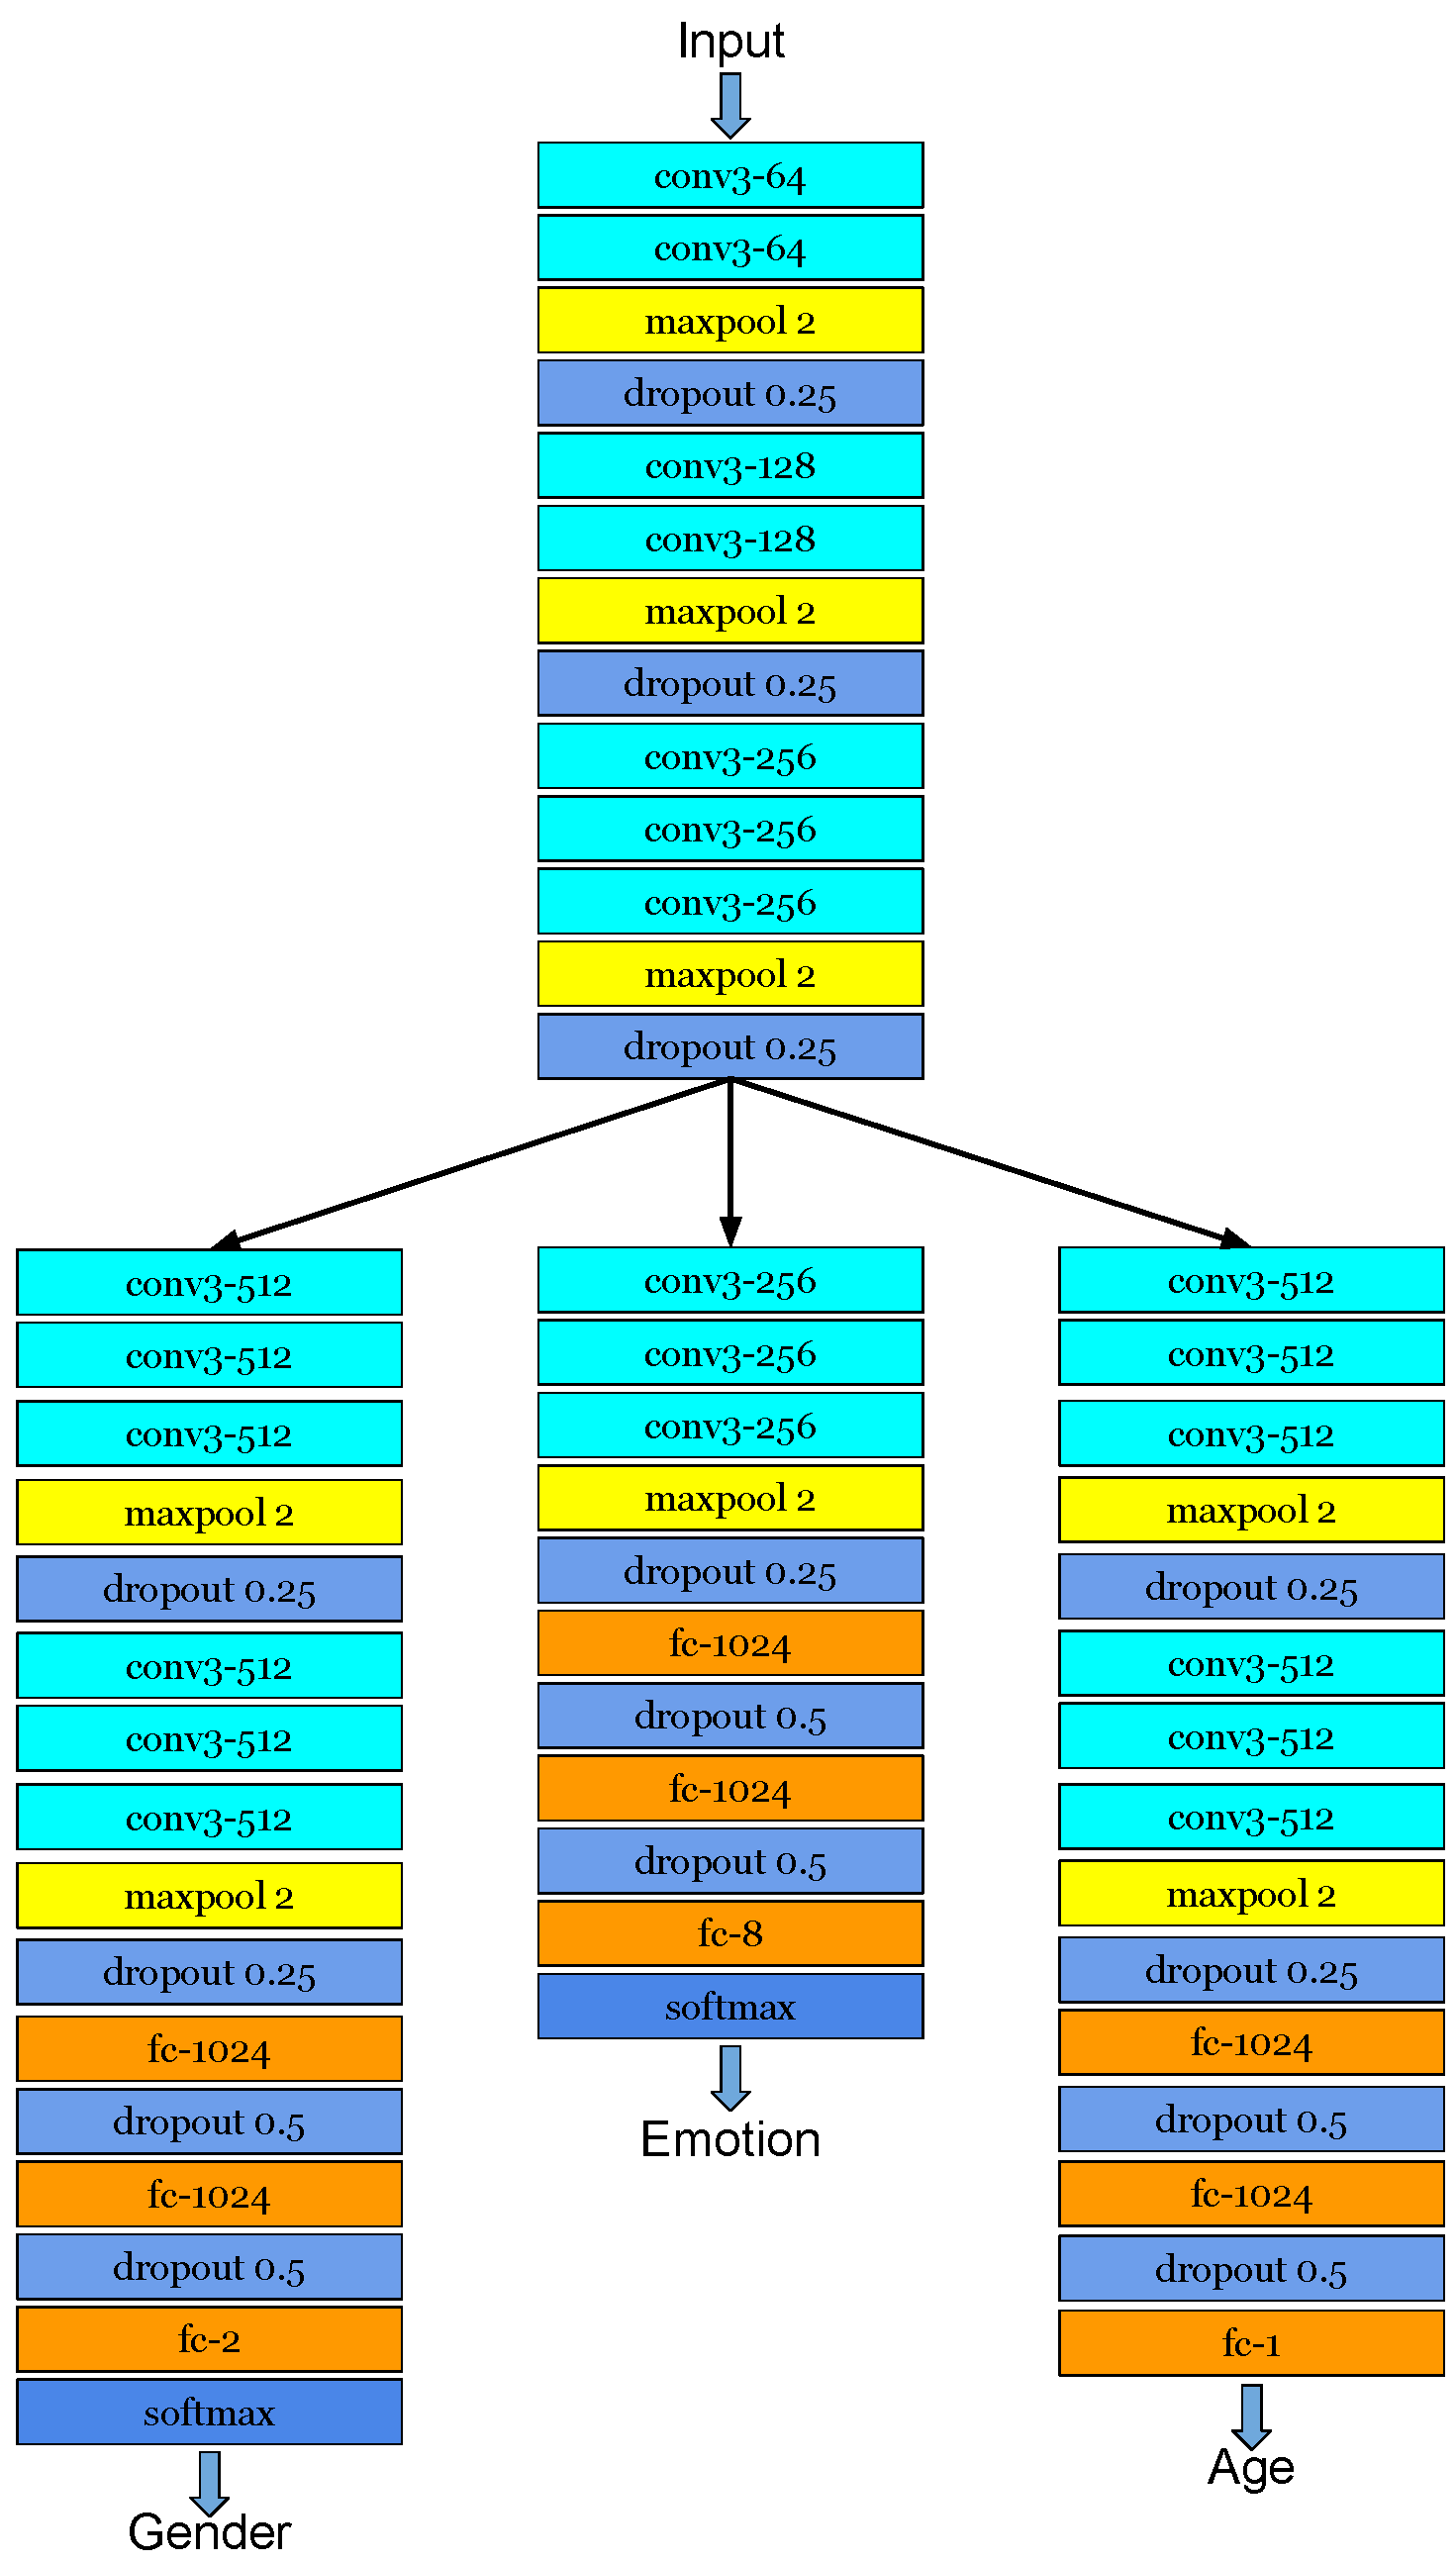
\includegraphics[width=0.8\textwidth]{images/multitask_real_1.pdf}
    \end{center}
    \caption{Multi-task learning} \label{fig:multitask_real_1}
\end{figure}

\begin{table}[]
\centering
\begin{tabular}{cc}
\hline
\multicolumn{2}{c}{\textbf{CNN}}          \\ \hline
\textbf{Architecture} & \textbf{Accuracy} \\ \hline
VGG13                 & 84.45             \\ \hline
VGG16                 & 84.43             \\ \hline
VGG19                 & 84.2              \\ \hline
ResNet18              & 82.57             \\ \hline
ResNet34              & 82.82             \\ \hline
ResNet50              & 82.37             \\ \hline
GoogLeNet             & 35.64             \\ \hline
DenseNet              & -                 \\ \hline
Wide ResNet           & \textbf{86.3}     \\ \hline
\end{tabular}
\caption{Accuracies from Convolutional Neural Networks}
\label{tab:cnn_accuracies}
\end{table}

\begin{table}[]
\centering
\begin{tabular}{cc}
\hline
\multicolumn{2}{c}{\textbf{Transfer Learning}}                                                                   \\ \hline
\textbf{Architecture}                                                                        & \textbf{Accuracy} \\ \hline
\begin{tabular}[c]{@{}c@{}}Fine-tuning\\ VGG16, ImageNet, conv3\_3\end{tabular}              & 46.39             \\ \hline
\begin{tabular}[c]{@{}c@{}}Fine-tuning\\ VGG16, ImageNet, conv4\_3\end{tabular}              & 42.21             \\ \hline
\begin{tabular}[c]{@{}c@{}}Fine-tuning\\ VGG16, Face Recognition, conv3\_3\end{tabular}      & \textbf{53.52}    \\ \hline
\begin{tabular}[c]{@{}c@{}}Fine-tuning\\ VGG16, Face Recognition, conv4\_3\end{tabular}      & 45.67             \\ \hline
\begin{tabular}[c]{@{}c@{}}fc6 Convolutional features\\ VGG16, ImageNet\end{tabular}         & 34.22             \\ \hline
\begin{tabular}[c]{@{}c@{}}fc7 Convolutional features\\ VGG16, ImageNet\end{tabular}         & 29.25             \\ \hline
\begin{tabular}[c]{@{}c@{}}fc6 Convolutional features\\ VGG16, Face Recognition\end{tabular} & 27.2              \\ \hline
\begin{tabular}[c]{@{}c@{}}fc7 Convolutional features\\ VGG16, Face Recognition\end{tabular} & 23.1              \\ \hline
\begin{tabular}[c]{@{}c@{}}ResNet50, ImageNet\end{tabular} & 21.13              
\\ \hline
\begin{tabular}[c]{@{}c@{}}InceptionV3, ImageNet\end{tabular} & 19.14              
\\ \hline
\end{tabular}
\caption{Accuracies from Transfer Learning}
\label{tab:transfer_learning_accuracies}
\end{table}

\begin{table}[]
\centering
\begin{tabular}{cc}
\hline
\multicolumn{2}{c}{\textbf{Multi-task Learning}}   \\ \hline
\textbf{Architecture}          & \textbf{Accuracy} \\ \hline
3 Tasks (Emotion, Gender, Age) & 85.2              \\ \hline
\end{tabular}
\caption{Accuracy from Multi-task learning}
\label{tab:multitask_learning}
\end{table}

